\documentclass{beamer}
\usetheme[pageofpages=de,% String used between the current page and the
                         % total page count.
          bullet=circle,% Use circles instead of squares for bullets.
          titleline=true,% Show a line below the frame title.
          alternativetitlepage=true,% Use the fancy title page.
          titlepagelogo=../img/fse_ministerio_ancho_texto.png%,% Logo for the first page.
	  %watermark=junta_girado,
          %watermarkheight=75px,% Height of the watermark.
          %watermarkheightmult=4,% The watermark image is 4 times bigger
                                % than watermarkheight.
          ]{Torino}

\usepackage[spanish]{babel} % Para separar correctamente las palabras
\usepackage[utf8]{inputenc} % Este paquete permite poner acentos y eñes usando codificación utf-8

\usepackage{color}

\author{IES Gonzalo Nazareno\\
IES Los Albares\\
IES La Campiña\\
IES Ingeniero de la Cierva}
\title{Introducción a Horizon}
\institute{Proyecto de Innovación\\ {\color{white} .\\} \emph{Implantación y
    puesta a punto de la infraestructura de un cloud computing privado para el
    despliegue de servicios en la nube}} 


\begin{document}
\begin{frame}[t,plain]
\titlepage
\end{frame}

\begin{frame}
  \frametitle{Horizon}
  \begin{itemize}
  \item Horizon es el panel de control web (\textit{dashboard}) de OpenStack
  \item Es una aplicación web desarrollada en Django
  \item Implementa las funcionalidades básicas de los componentes principales de
    OpenStack: Nova, Glance, Swift, etc. 
  \item Permite utilizar fácilmente OpenStack mediante una interfaz web simple
  \item Como todos los componentes de OpenStack está sometida a un fuerte
    desarrollo, por lo que cambia bastante con cada versión.
  \item Utilizamos Horizon para OpenStack Essex (2012.1)
  \end{itemize}
\end{frame}

\begin{frame}
  \frametitle{Acceso a Horizon}
  \begin{columns}
    \column{.7\textwidth}
    \begin{itemize}
    \item Acceso mediante usuario/contraseña
    \item Dos roles predefinidos: admin y member
    \item Un usuario con el rol member puede:
      \begin{itemize}
      \item Crear instancias
      \item Modificar el estado de sus instancias
      \item Adquirir direcciones IP públicas
      \item Asociar direcciones IP públicas a sus instancias
      \item Crear y editar reglas de acceso a sus instancias mediante los Grupos
        de Seguridad 
      \item Crear pares de clave ssh y asociarlas a instancias
      \end{itemize}
    \end{itemize}
    \column{.3\textwidth}
    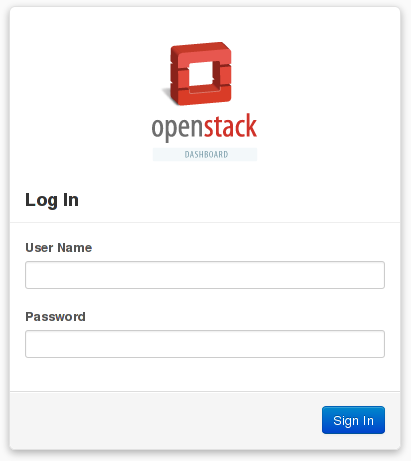
\includegraphics[width=\columnwidth]{../img/horizon1.png}
  \end{columns}
\end{frame}

\begin{frame}
  \frametitle{Conceptos previos}
  \begin{description}
  \item[Imagen] Imagen de sistema preconfigurado que se utiliza como base para
    crear instancias. Dentro del cloud habrá diferentes imágenes para cada tipo
    de instacia que se quiera utilizar. 
  \item[Instancia] Clon de una imagen que se crea a demanda del usuario en uno
    de los nodos del cloud.
  \item[IP privada] Dirección IP con la que se crean las instancias y que se
    utiliza para comunicación interna. 
  \item[IP flotante] Dirección IP pública que puede asociarse a diferentes
    instancias con el fin de acceder a ellas desde fuera. 
  \item [Grupo de seguridad] Reglas de cortafuegos (iptables) que controlan el
    acceso a las instancias mediante la dirección IP flotante. 
  \item[Par de claves ssh] Utilizadas para acceder por ssh a las instancias
    desde fuera del cloud.
  \end{description}
\end{frame}

\begin{frame}
  \frametitle{Acceso inicial}
  \begin{columns}
    \column{.7\textwidth}
    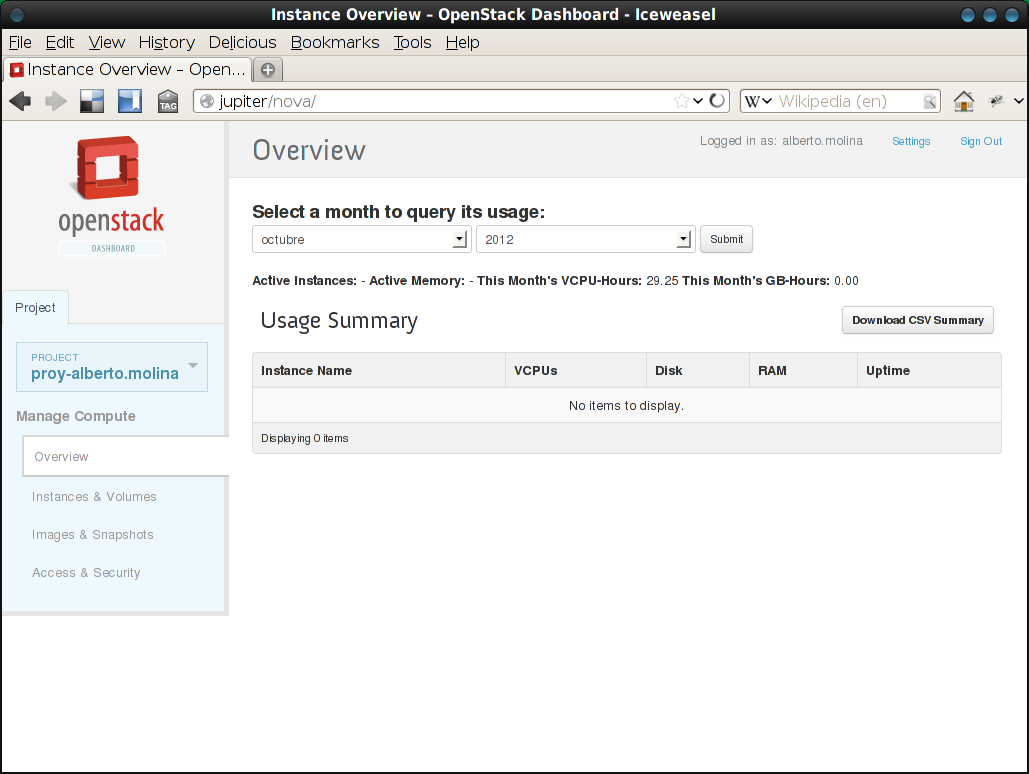
\includegraphics[width=\columnwidth]{../img/horizon2.png}
    \column{.35\textwidth}
    \begin{itemize}
    \item Un usuario puede pertenecer a diferentes proyectos
    \item Sencillo menú que muestra las acciones a realizar
    \end{itemize}
  \end{columns}
\end{frame}

\begin{frame}
  \frametitle{Grupo de Seguridad (I)}
  \begin{itemize}
  \item Es posible definir diferentes grupos de seguridad (conjunto de reglas de
    cortafuegos) para aplicar a las instancias de cada proyecto.
  \item Accedemos al menú \textit{Access \& Security} y editamos las reglas del
    grupo \textit{default} de la sección \textit{Security Groups}
  \end{itemize}
  \begin{center}
    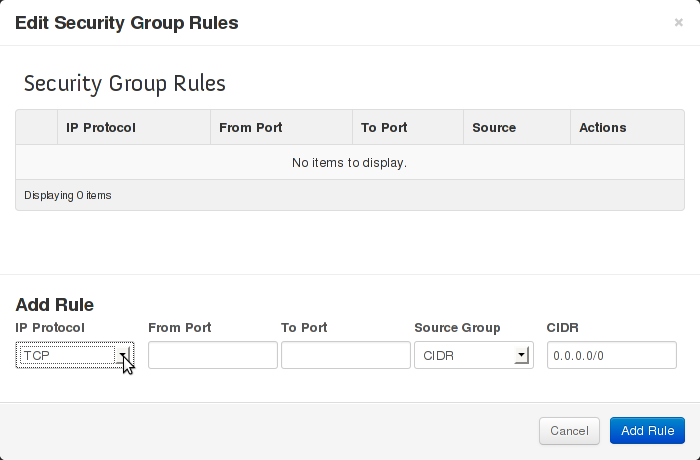
\includegraphics[width=.5\textwidth]{../img/horizon3.png}    
  \end{center}

\end{frame}

\begin{frame}
  \frametitle{Grupo de Seguridad (II)}
  \begin{itemize}
  \item Inicialmente permitimos conexiones a las instancias de este grupo
    mediante ssh (22/tcp)
  \item Permitimos el protocolo ICMP completo para peticiones realizadas desde
    el exterior a estas instancias.
  \end{itemize}
  \begin{center}
    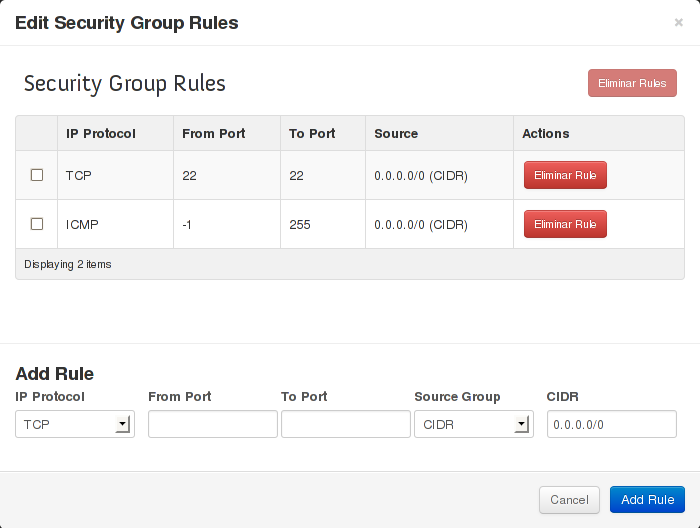
\includegraphics[width=.5\textwidth]{../img/horizon4.png}  
  \end{center}
\end{frame}

\begin{frame}[fragile]
  \frametitle{Pares de clave ssh}
  \begin{itemize}
  \item Inicialmente no sabemos el usuario/contraseña para acceder a la
    instancia (por seguridad no deberían tener contraseña definida porque sería
    igual para todas las instancias del cloud)
  \item Se utilizan pares de claves pública/privada RSA para acceder por ssh sin
    contraseña. 
  \item Cuando se lanza la instancia se puede inyectar la clave pública RSA que
    se elija $\Rightarrow$ Sólo el usuario que tenga la clave privada RSA podrá
    acceder.
  \item En la sección \textit{Keypairs} de \textit{Access \& Security} podemos
    crear un par de claves RSA. La clave pública se quedará almacenada y se nos
    descargará la privada.
  \item Hay que proteger adecuadamente la clave privada:
\begin{verbatim}
$ mv ~/Descargas/clave-prueba.pem ~/.ssh
$ chmod 400 ~/.ssh/clave-prueba.pem
\end{verbatim}
  \end{itemize}
\end{frame}

\begin{frame}
  \frametitle{Lanzar instancias (I)}
  \begin{columns}
    \column{.7\textwidth}
    \begin{center}
      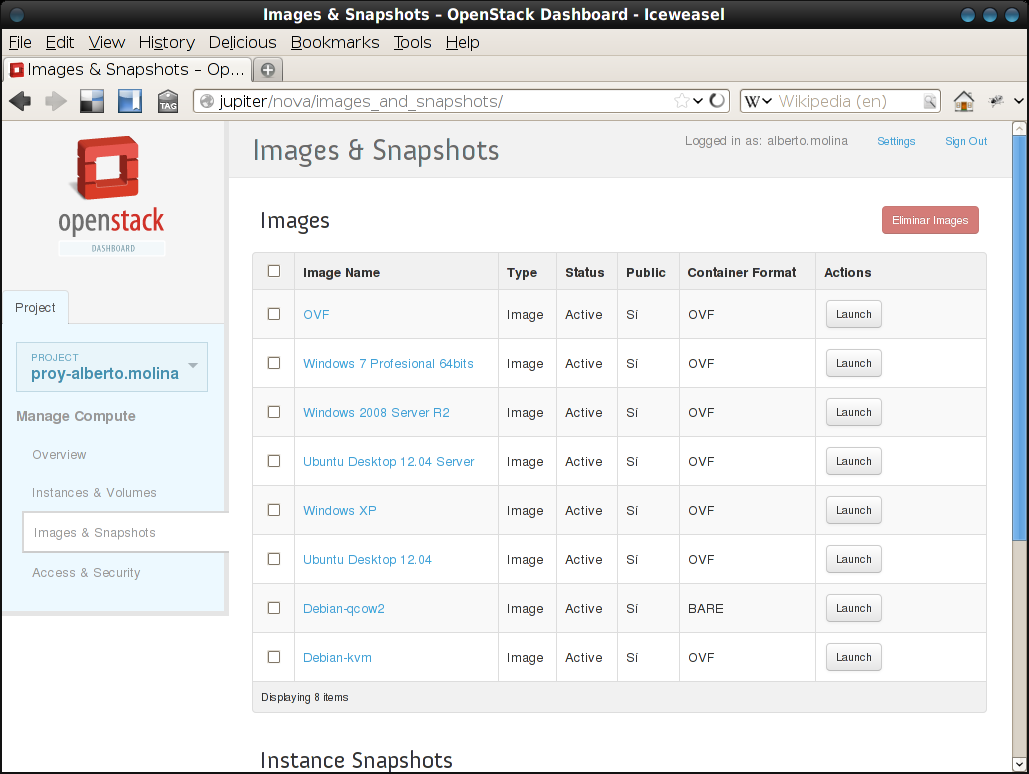
\includegraphics[width=\columnwidth]{../img/horizon5.png}
    \end{center}
    \column{.35\textwidth}
    \begin{itemize}
    \item Menú \textit{Images \& Snapshots}
    \item Seleccionamos la imagen adecuada y pulsamos sobre \textit{Launch}
    \end{itemize}
  \end{columns}
\end{frame}

\begin{frame}
  \frametitle{Lanzar instancias (II)}
  \begin{columns}
    \column{.6\textwidth}
    \begin{center}
      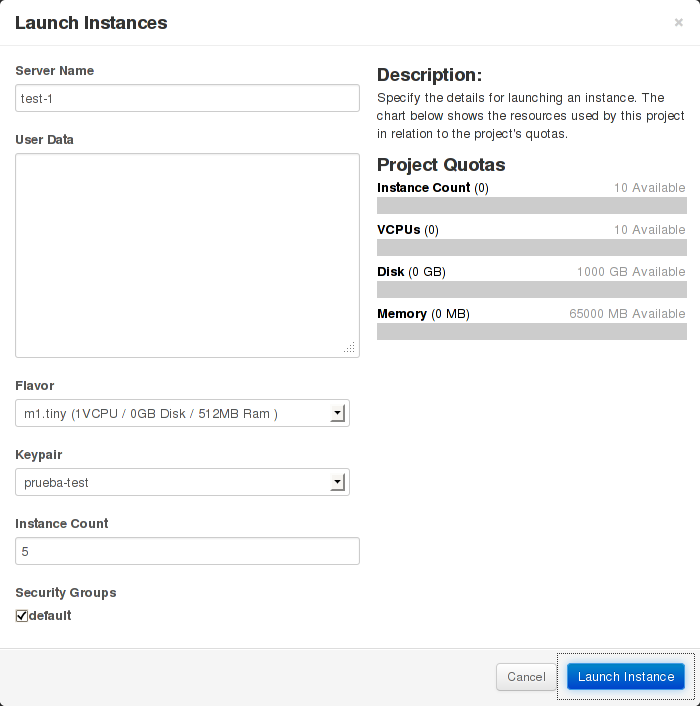
\includegraphics[width=.8\columnwidth]{../img/horizon6.png}      
    \end{center}
    \column{.4\textwidth}
    Seleccionamos:
    \begin{itemize}
    \item Nombre de la instancia
    \item Sabor (\textit{flavor})
    \item Par de claves ssh
    \item Grupo de seguridad
    \item Número de instancias iguales
    \end{itemize}
  \end{columns}
\end{frame}

\begin{frame}
  \frametitle{Lanzar instancias (III)}
  \begin{itemize}
  \item Se van levantando las instancias en los nodos del cloud:
  \end{itemize}
  \begin{center}
    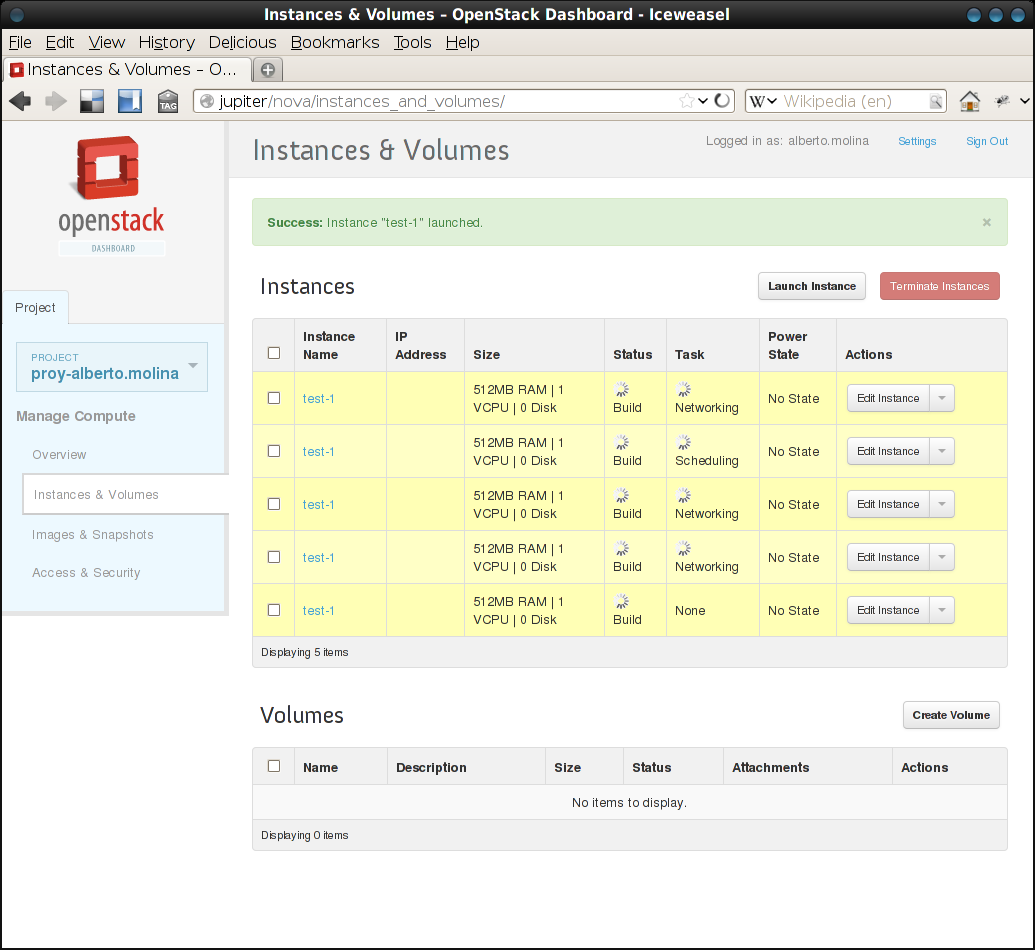
\includegraphics[width=.6\textwidth]{../img/horizon7.png}    
  \end{center}
\end{frame}

\begin{frame}
  \frametitle{Lanzar instancias (IV)}
  \begin{itemize}
  \item Finalmente termina el lanzamiento y las instancias son ya operativas:
  \end{itemize}
  \begin{center}
    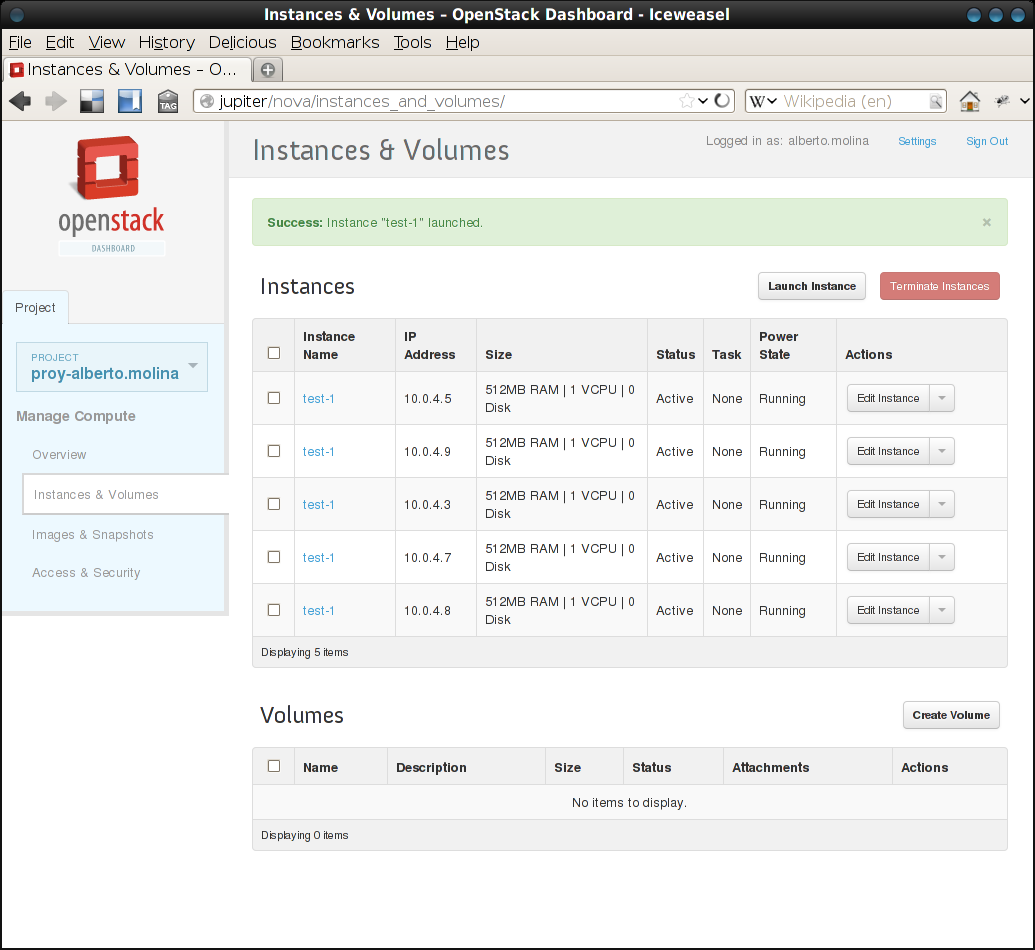
\includegraphics[width=.6\textwidth]{../img/horizon8.png}
  \end{center}
\end{frame}

\begin{frame}
  \frametitle{Asociación de IP flotante}
  \begin{itemize}
  \item Las direcciones IP asignadas se denominan privadas porque son sólo para
    comunicación interna (en el ejemplo las 10.0.4.X)
  \item Para poder acceder a un equipo del cloud desde fuera es necesario
    asociarle una dirección IP flotante (en el ejemplo las 172.22.122.X)
  \end{itemize}
  \begin{columns}
    \column{.5\textwidth}
    \begin{itemize}
    \item En \textit{Access \& Security} vamos a la sección \textit{Floating
        IPs} y asignamos una IP al proyecto.
    \item Seleccionamos la dirección IP flotante y la asociamos a una de las
      instancias lanzadas
    \item Repetimos el proceso con el resto de instancias
    \end{itemize}
    \column{.5\textwidth}
    \begin{center}
      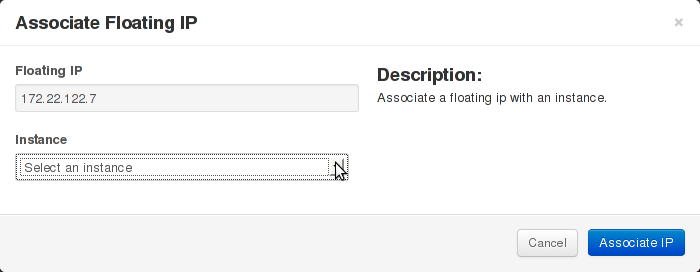
\includegraphics[width=\columnwidth]{../img/horizon9.png}
    \end{center}
  \end{columns}
\end{frame}

\begin{frame}
  \frametitle{Acceso a la instancia (I)}
  \begin{itemize}
  \item Comprobamos la conectividad con la instancia a través de la IP flotante asociada:
  \end{itemize}
  \begin{center}
    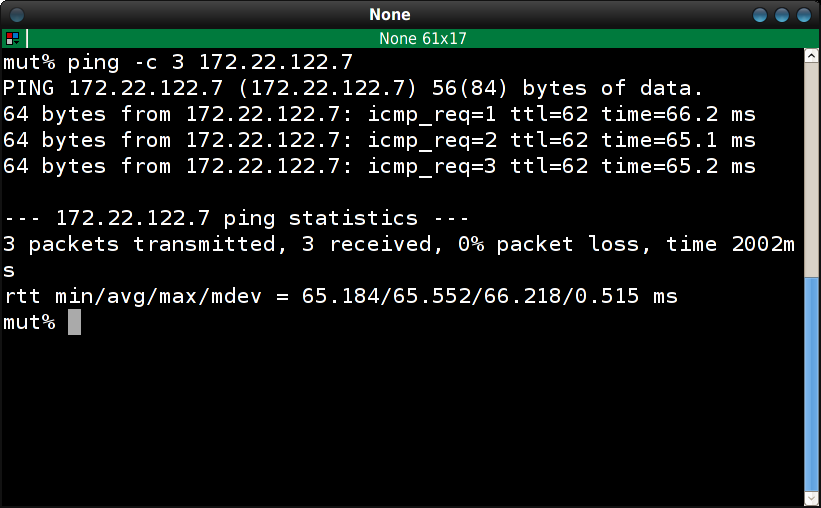
\includegraphics[width=.7\textwidth]{../img/horizon10.png}    
  \end{center}
\end{frame}

\begin{frame}[fragile]
  \frametitle{Acceso a la instancia (II)}
  \begin{itemize}
  \item Finalmente accedemos a la instancia por ssh utilizando la clave RSA privada:
  \end{itemize}
  \begin{center}
    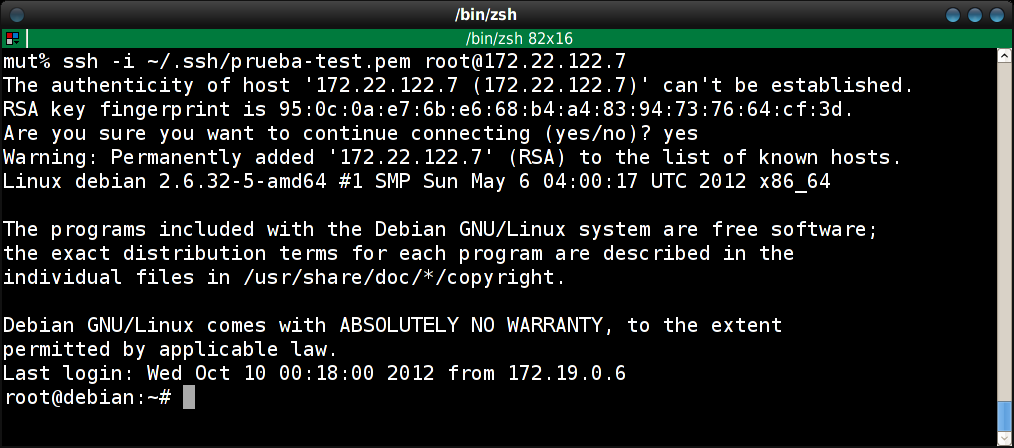
\includegraphics[width=.8\textwidth]{../img/horizon11.png}
  \end{center}
\end{frame}
\end{document}
